\section{Results}
\label{sec:bw:results}

In each EAToF measurement, an ultrasonic pulse is incident on the battery being tested. As the initial pulse passes through each interface, some fraction of the wave is transmitted and some is reflected, depending on the degree of mismatch in the sound speed c between adjacent layers and whether c increases or decreases from one layer to the next; additionally, the wave attenuates (i.e., loses energy) as it passes through the bulk region of each layer.~\cite{Cheeke2012-wp} As each interface is an opportunity for the pulse to split, as the acoustic behavior of the cell quickly becomes complicated as each new wave interacts not only with interfaces (creating even more waves) but also with each other. The complex interplay of sound speed mismatches as well as constructive and destructive interference between the waves creates the observed reflection and transmission traces which are shown in this chapter. Furthermore, as the time of flight (ToF) increases, the sound waves become increasingly dampened due to dissipation and the increasing number of encountered interfaces. The result is an “echo chamber" effect for the longer ToF waves.

\subsection{Simulation}
To simulate the effect of galvanostatic cycling on the echoing behavior of the cell, a simple 1D stack of the regions listed in Table~\ref{tab:bwtab1} was created in the standard cell geometry defined by Dualfoil.~\cite{Albertus2007-eu} For a series of time steps, the changes in electrode densities were calculated as a function of SOC using Dualfoil, which were then fed into Clawpack to determine the resulting acoustic behavior of the cell. The snapshots were composited to obtain the time-resolved simulated acoustic results shown in Fig.~\ref{fig:lionsim}. This simulation illustrates that during cycling, there is a measurable shift in the ToF of the primary transmission gauge reading (indicated by arrow 1) as well as a change in the signal intensity, which are both clearly functions of the SOC of the battery (i.e., density changes in the anode and cathode due to lithium intercalation/deintercalation). In addition to becoming increasingly dampened, the later transmission signals (e.g., the trace indicated by arrow 2) display an enhanced shift in ToF between the charged and discharged states. Similar trends are observed in the reflection data.

\begin{figure}[htb]
  \centering
    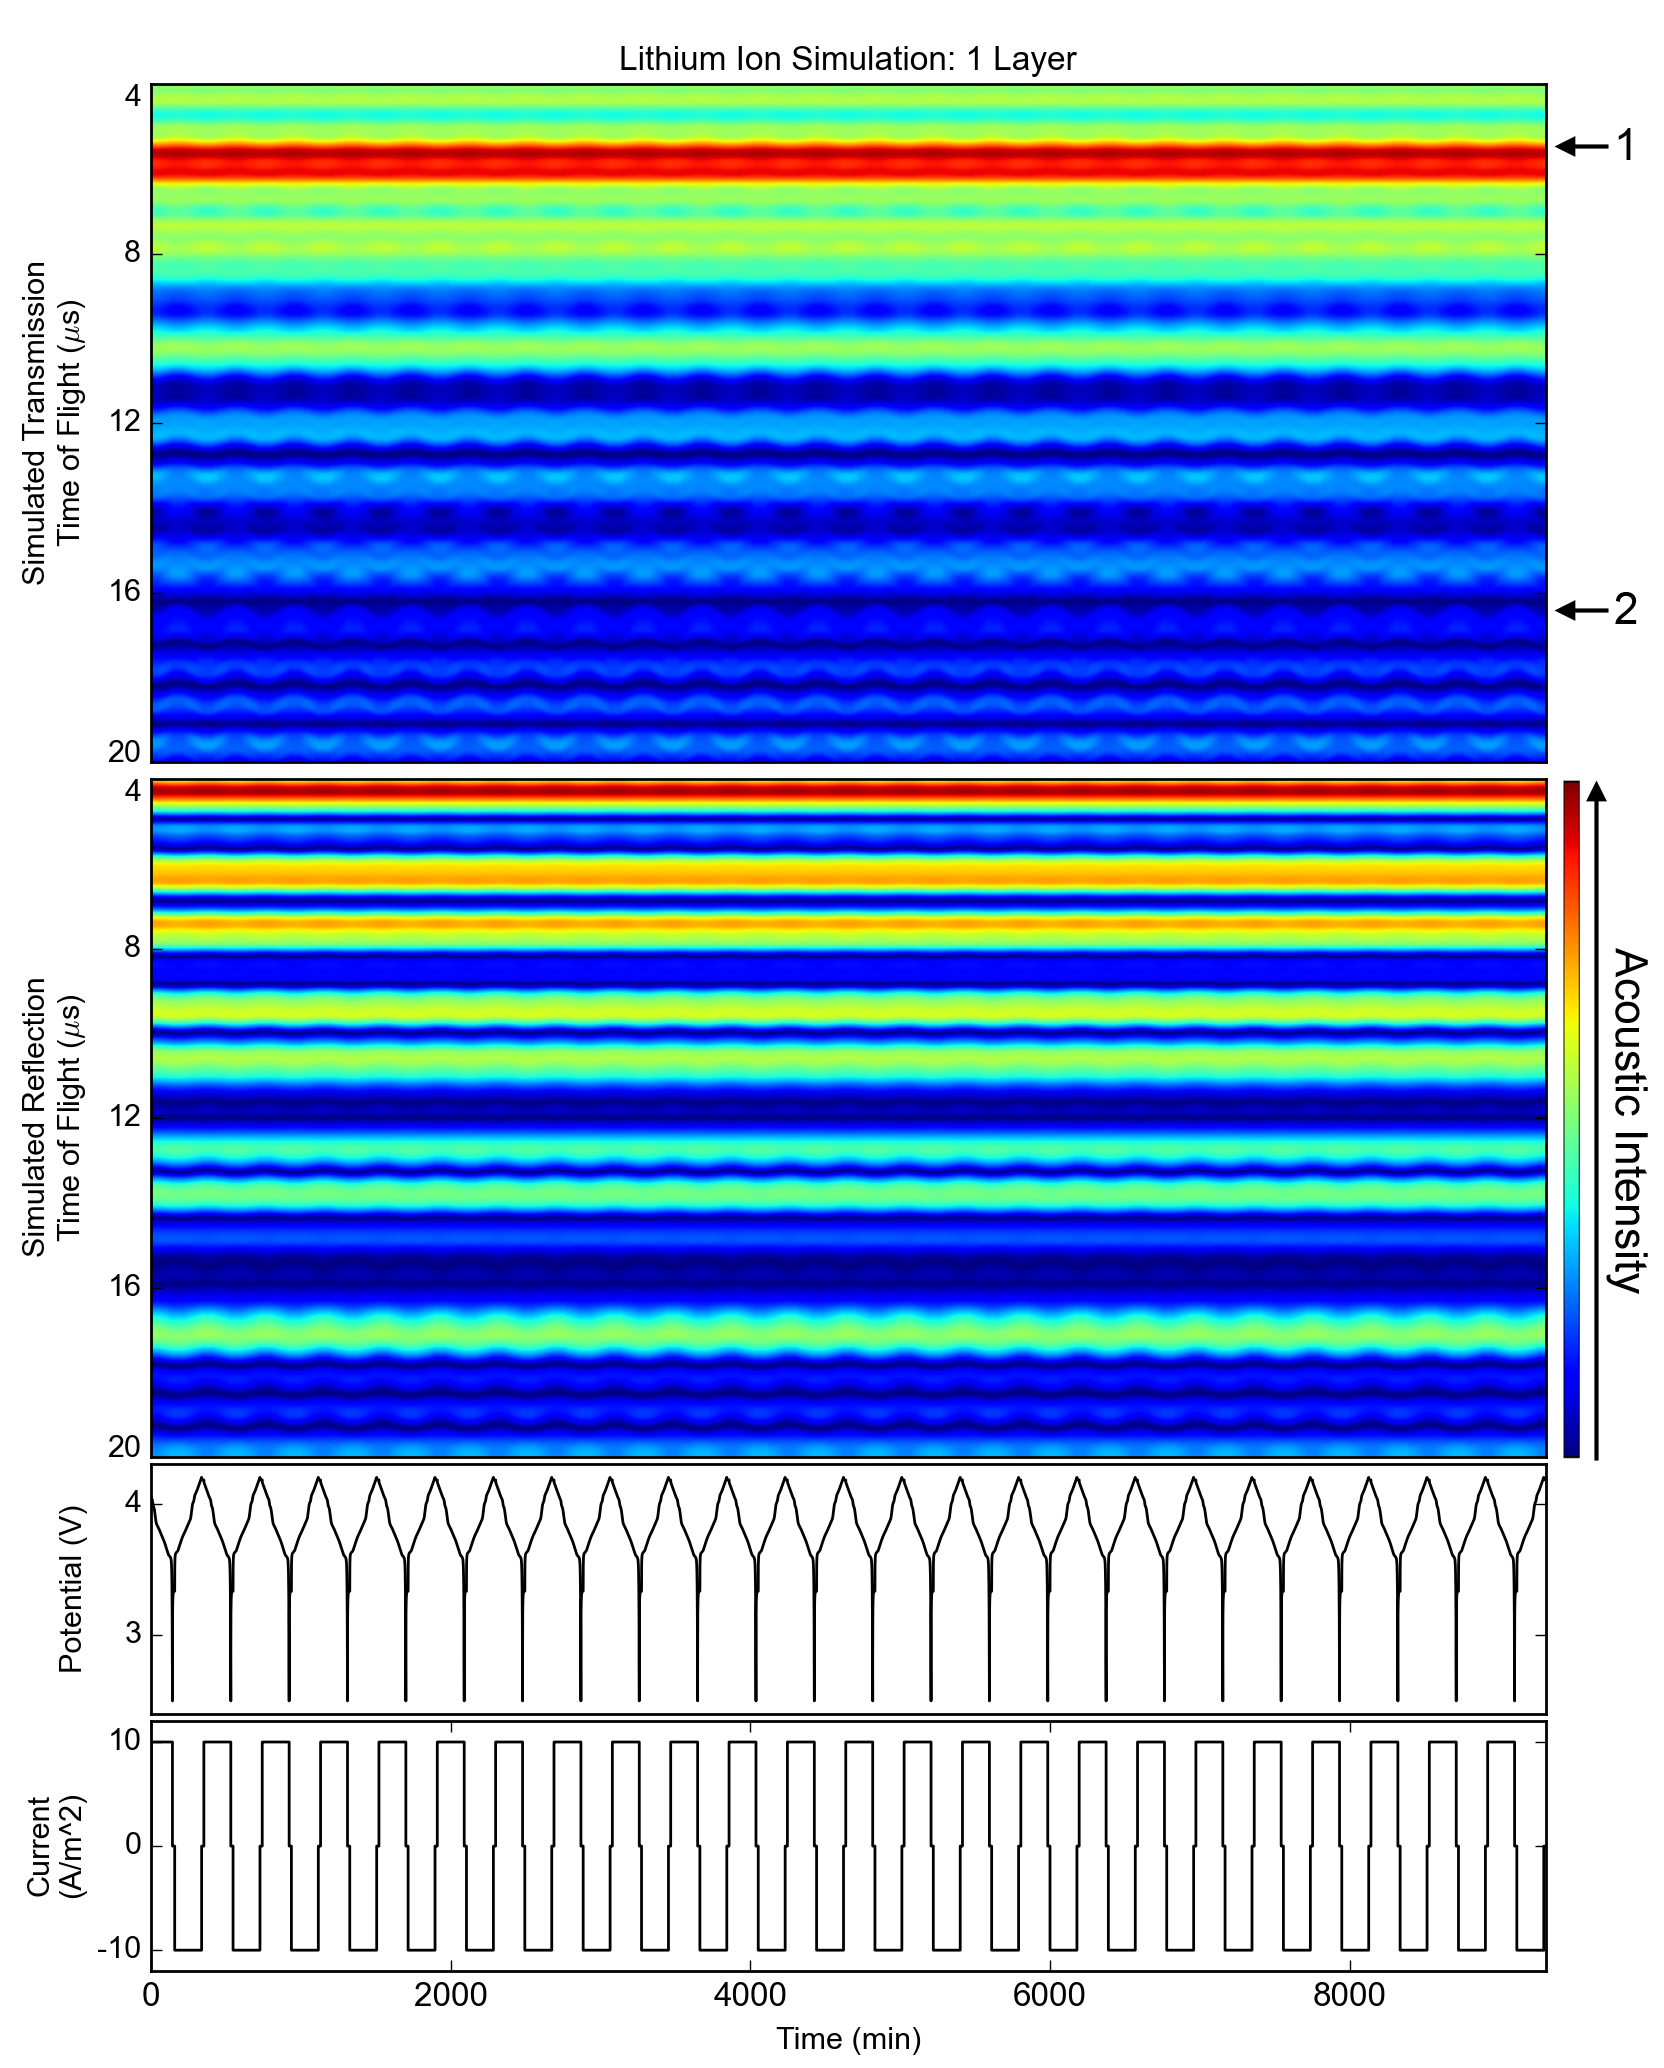
\includegraphics[width=0.8\textwidth]{ch4-bw/images/lionsim.png}
    \caption[Simulation of echo behavior as a function of SOC.]{Simulation of transmission and reflection behavior as a function of SOC, and cell potential and applied current density profiles. Color bar denotes signal intensity.}
    \label{fig:lionsim}
\end{figure}

To simulate cylindrical and prismatic cell designs, cells consisting of multiple stacks of electrodes were run through the Clawpack-Dualfoil simulation, and Fig.~\ref{fig:multistack} demonstrates the effect of cell folding/winding on the output acoustic signals. We see that as the size of the simulated cell is increased to 4 electrode stacks, the acoustic behavior becomes increasingly complex, as there are more and more interfaces for the waves to pass through, resulting in a progressively increasing number of waves echoing and interfering with one another. It is worth noting that commercially available cells generally contain many more layers than this, which, as we will see further below, results in even more complex acoustic behaviors.

\figskip{fig:multistack}

\begin{figure}[htb]
  \centering
    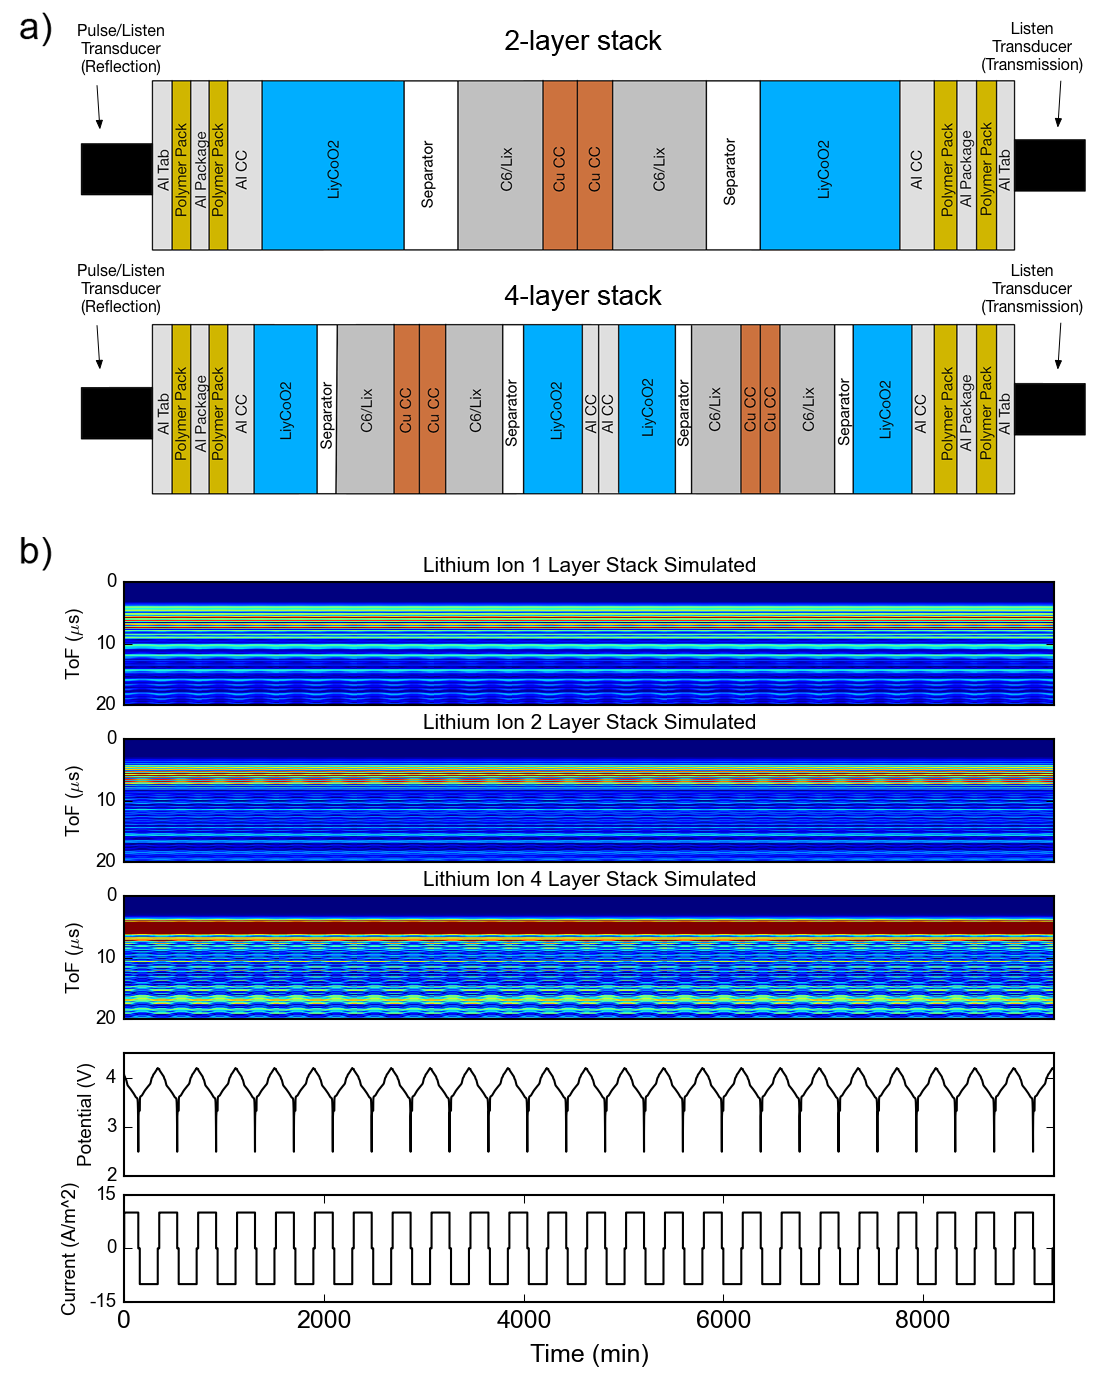
\includegraphics[width=\textwidth]{ch4-bw/images/multistack.png}
    \caption[Simulated effect of multiple layers on ToF signal.]{Simulated effect of multiple layers on ToF signal as a function of SOC, and cell potential and applied current density profiles. Color bar denotes signal intensity.}
    \label{fig:multistack}
\end{figure}

\clearpage

\subsection{Ultrasonic ToF analysis of~\ce{LiCoO2}/graphite pouch cell}
Ultrasonic time of flight analysis was performed on a commercial~\ce{LiCoO2}/graphite pouch cell during galvanostatic cycling: the reflected and transmitted signals were measured every 30 seconds during cycling, providing acoustic snapshots of the cell as a function of time. Time-resolved acoustic results were visualized by compositing these snapshots into a two-dimensional intensity image of cycle time against ToF data (selected data shown in Fig.~\ref{fig:lco}a and~\ref{fig:lco}b, full data set shown in Fig.~\ref{fig:lcofull}). These composite images demonstrate both the change in intensity for each acoustic wave received by the transducers as well as the ToF shift in each wave during cycling. Focusing on the transmission data (Fig.~\ref{fig:lco}a), we see that each ToF peak shifts towards lower values and higher intensities during charge, and towards higher values and lower intensities during discharge. Furthermore, a comparison of transmission peaks 1, 3, and 10 shows that the later (i.e., longer ToF) peaks display a more pronounced shift in ToF position between the charged and discharged states, and are in general less intense. Similar trends are also observed in the reflection data (Fig.~\ref{fig:lco}b). These experimental trends are reminiscent of the shifts in ToF and intensity observed in the Clawpack-Dualfoil simulations. While there are strong correlations between the simulated SOC-ToF relationship and the overall experimental ToF trends, due to the assumptions made, our model does not capture many of the nonlinear intercalation-driven changes that are known to occur. Nevertheless, we are able to draw several meaningful correlations between the acoustic and electrochemical results.

\begin{figure}[htb]
  \centering
    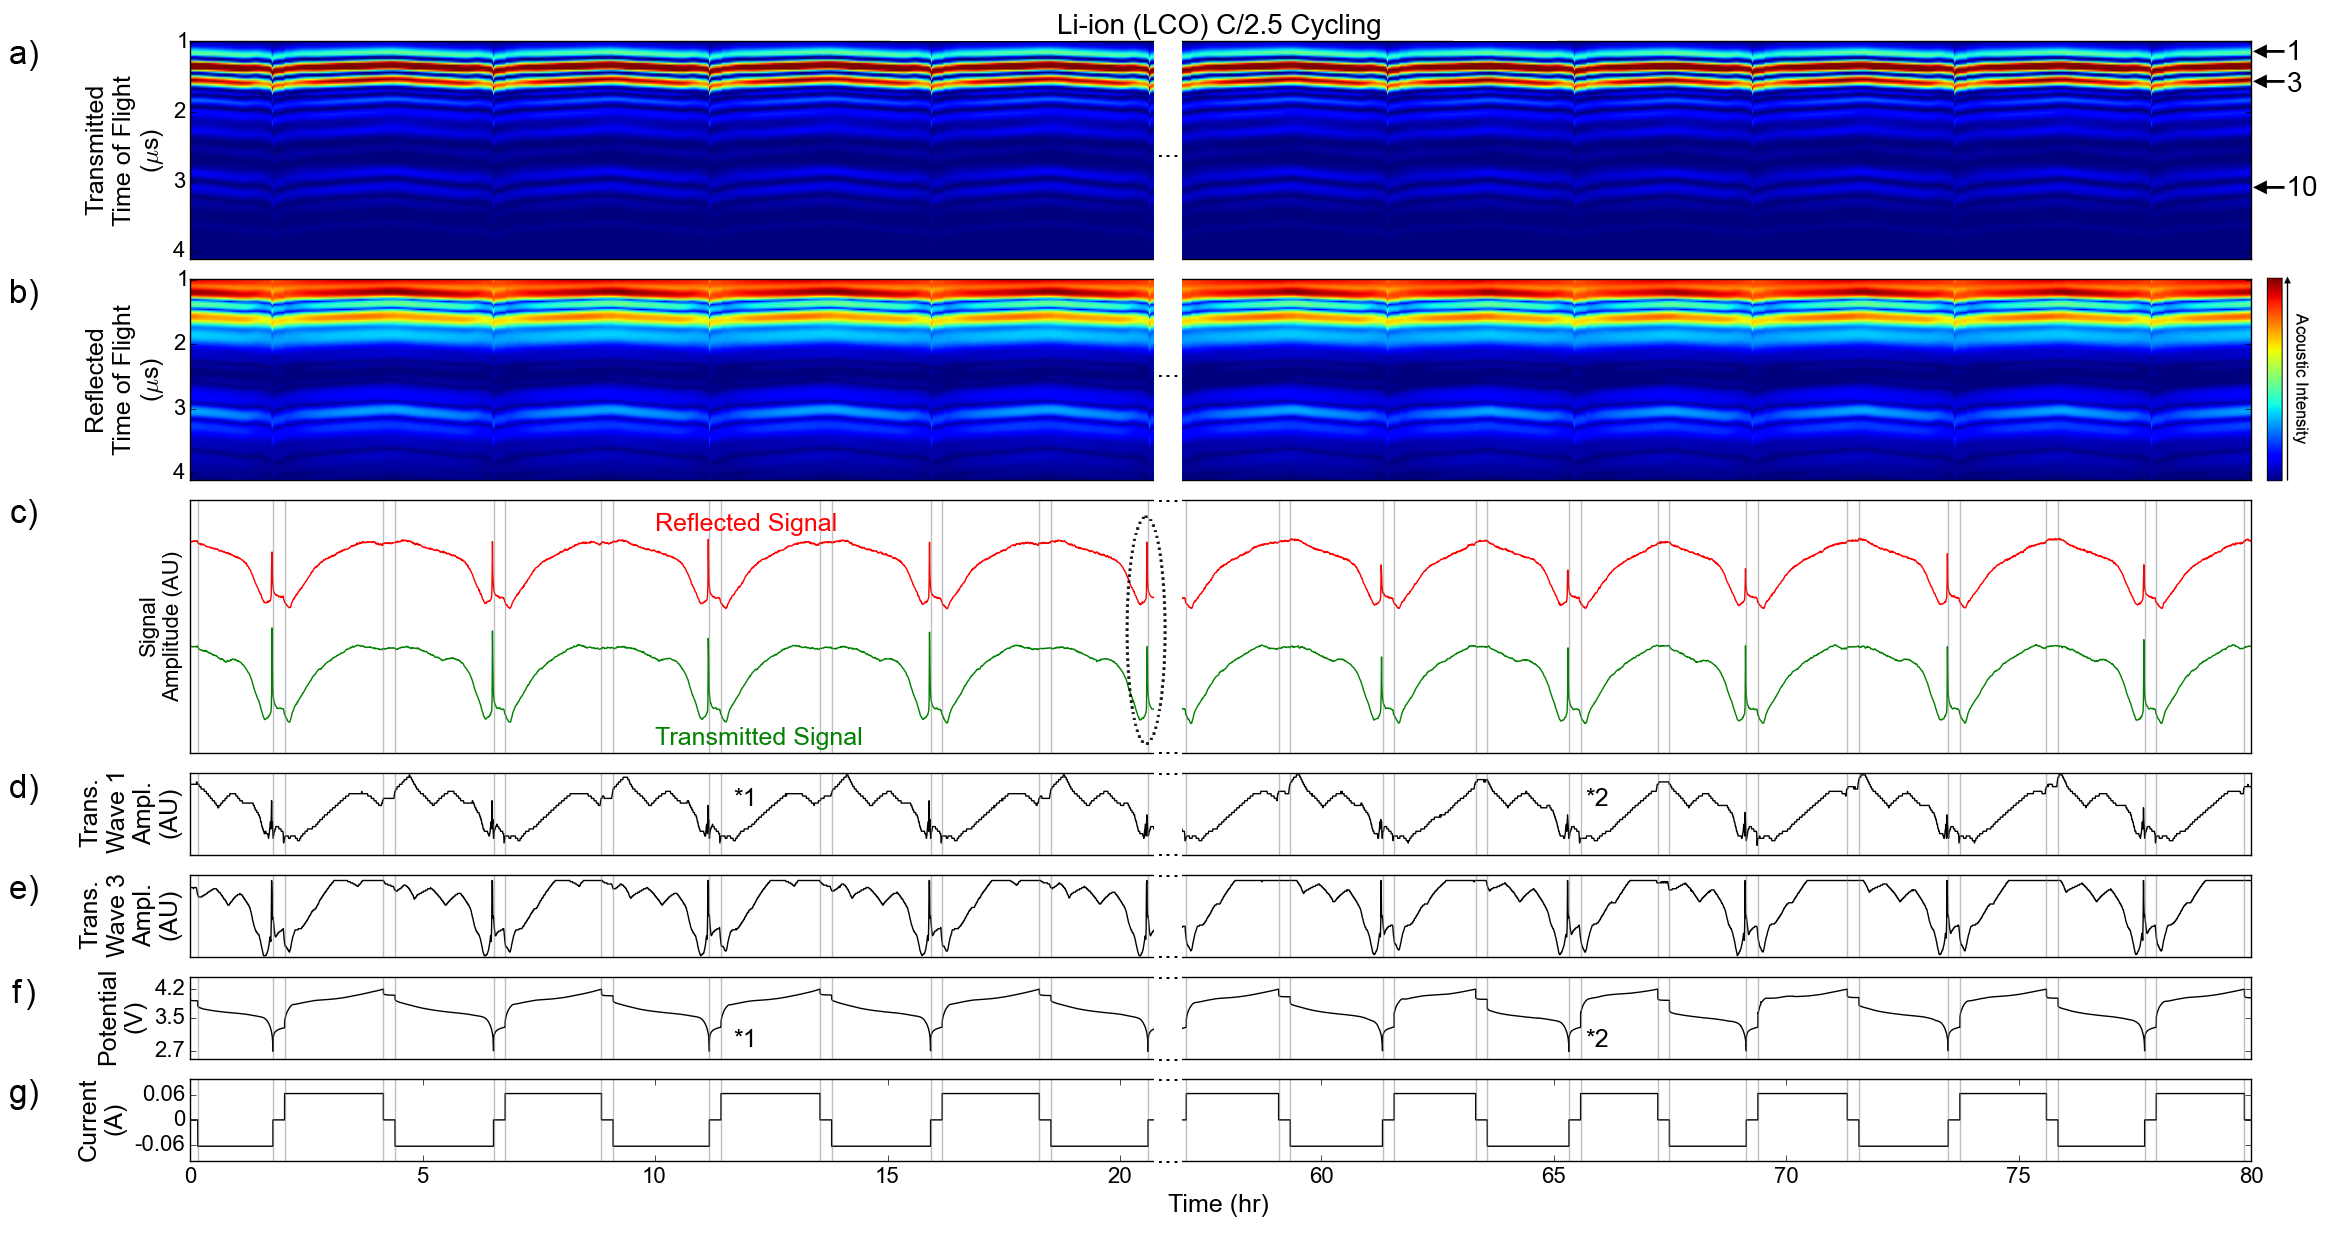
\includegraphics[width=\textwidth]{ch4-bw/images/lco.png}
    \caption[Acoustic behavior of a~\ce{LiCoO2}/graphite prismatic cell.]{Acoustic behavior of a~\ce{LiCoO2}/graphite prismatic cell. a,b) ToF maps for transmission and reflection modes, respectively, c) total reflected (red) and transmitted (green) signal amplitudes, d,e) traces for the amplitudes of transmitted waves 1 and 3, respectively, (f) cell potential, and g) applied current as a function of cycling time. The vertical gray lines in panels c-g represent transitions between charge, discharge, and rest steps; arrows 1, 3, and 10, the dotted oval, as well as markings *1 and *2 are discussed in the text.}
    \label{fig:lco}
\end{figure}

For each ToF snapshot, we calculated the total transmitted and reflected signal amplitudes by summing the intensity across the entire 0-20 µs ToF window, shown in Figure~\ref{fig:lco}c. As the battery is discharged, acoustic absorption increases (i.e., the transmitted and reflected intensities decrease), with a notable, but repeatable, exception at the end of discharge at a cell potential $<$ 3.5 V, where there is a dramatic increase in the signal intensities (dotted oval, Fig.~\ref{fig:lco}c). We believe this is driven primarily by the capacity-limited cathode: near 0\% SOC,~\ce{LiCoO2} approaches a hexagonal-to-monoclinic phase transformation, dramatically altering both the modulus and density of the cathode.~\cite{Reimers1992-ql} Following discharge, as the applied current is removed during the rest step, we see the cell potential increase as local lithium gradients relax, which in turn relaxes any build-up in lattice strain due to the aforementioned phase transformation, and the acoustic signal intensities decrease accordingly. When the cell is charged, the acoustic intensities decrease slightly as the phase transformation is reversed, followed by a steady increase in the intensities with increasing SOC. At the end of charge, there is a slight, repeatable increase in acoustic absorption when the cell potential is $>$ 4 V. We believe that this is also driven primarily by the cathode, as near 100\% SOC, the \ce{LiCoO2} undergoes a two-phase staging reaction which changes its density significantly.~\cite{Van_der_Ven1998-tq}
	
Particularly interesting is the information contained within individual ToF peak traces. Figures~\ref{fig:lco}d and~\ref{fig:lco}e show the amplitudes of Transmitted Waves 1 and 3, respectively, and we see that while their general trends are similar to one another and to the total amplitude, there are subtle differences between them. Furthermore, amplitude changes in the individual waves follow different trends with cycle number. For example, if we focus on the amplitude of Transmitted Wave 1 during the charge step, there is a peak in the 3rd cycle (marked by *1, Fig.~\ref{fig:lco}d) that disappears by the 15th cycle (*2, Fig.~\ref{fig:lco}d). These changes seem to be a strong predictor of the cell accepting less charge before the 4.2 V cut-off potential, evident from the respective potential profiles and charging times. We note that the cell recovered some capacity before continuing the trend toward degradation, and that similar types of correlations between amplitude and capacity can be made for other individual wave traces as well. While the changes are slight, comparison of the overall recovered acoustic signal with the signal recovered for specific ToF traces nevertheless reveals repeatable correlations with SOH. This is intriguing as it enables the development of detailed acoustic models in which hypothetical electrode degradation mechanisms can be compared to the performance of a practical cell. The development of such models is not a trivial endeavor and is currently under investigation.


\subsection{Ultrasonic ToF analysis of~\ce{Li(NiCoAl)O2}/graphite ``jelly roll" cell}

To evaluate the influence of cell construction and material distribution on acoustic behavior, ultrasonic ToF analysis was performed on a \ce{Li(NiCoAl)O2} (NCA)/graphite 18650 ``jelly roll" cell during galvanostatic cycling starting from a fresh state (selected data shown in Fig.~\ref{fig:nca}, full data set in Fig.~\ref{fig:ncafull}). As shown in the ToF maps (Fig.~\ref{fig:nca}a and b), the acoustic behavior is significantly more complicated in the 18650 cell than in the prismatic cell (Fig. 3). Based on the simulated ToF maps from Fig.~\ref{fig:multistack}, this increase in acoustic complexity is expected, as cells of this design typically consist of 15 to 25 layered windings.~\cite{linden} The total reflected and transmitted signal intensities (Fig.~\ref{fig:nca}c) as a function of SOC varies significantly over the first 11 cycles, after which the acoustic behavior stabilizes; this indicates the presence of an initial “formation" period, which is consistent with previous efforts on the acoustic emission of batteries.\cite{Komagata2010-sw,Rhodes2010-nr} As cycling continues, the total transmitted signal at the end of charge becomes increasingly large, as after ~27 cycles new peaks between 8 and 12 µs begin to appear in the transmission ToF map (Fig.~\ref{fig:nca}a, indicated by the white arrow).

\begin{figure}[htb]
  \centering
    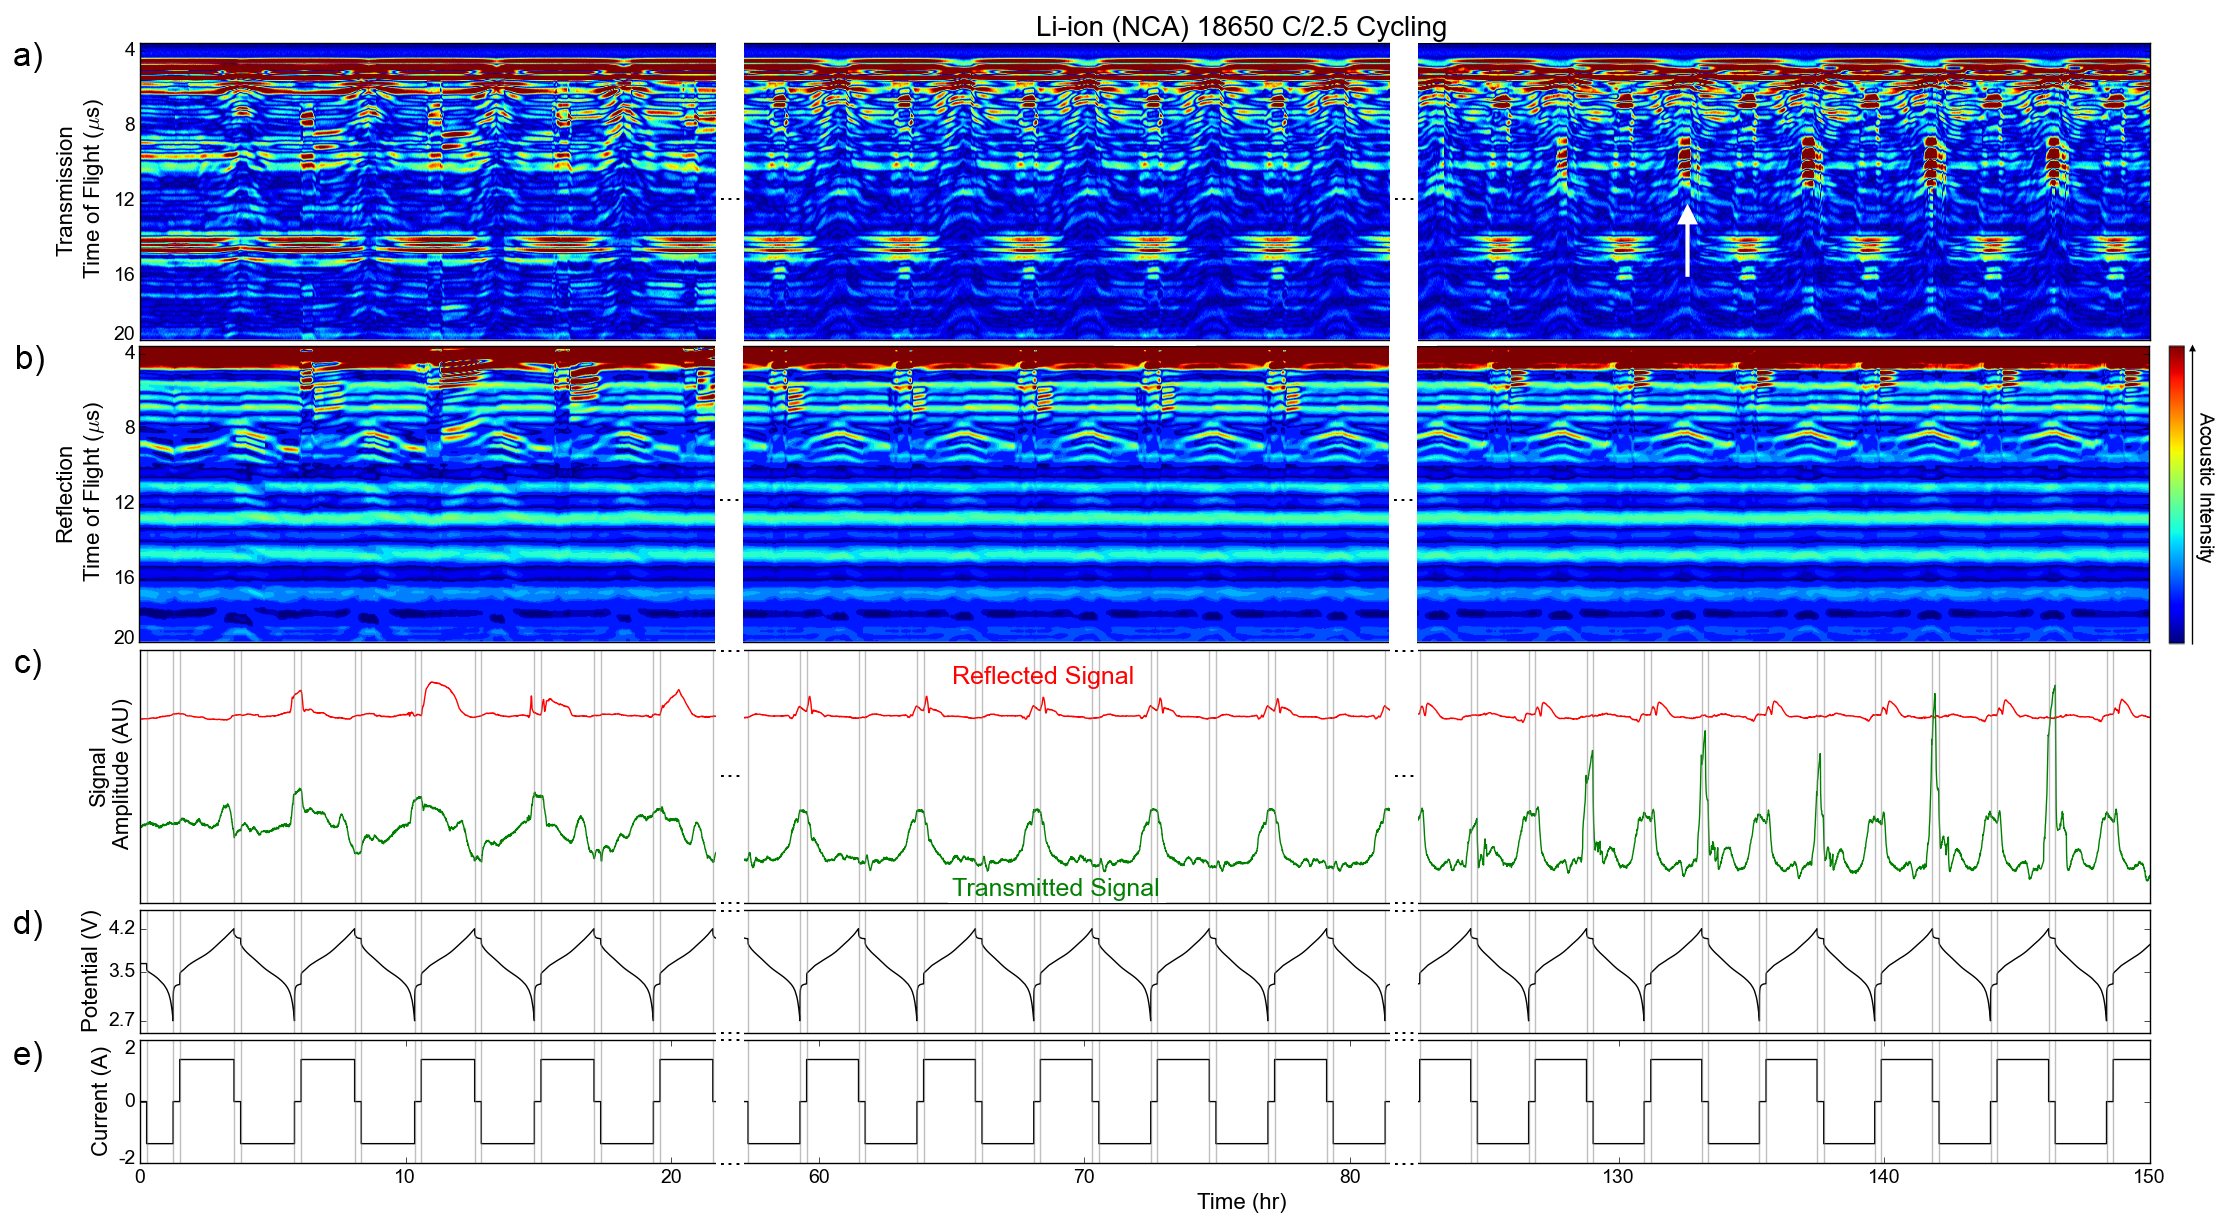
\includegraphics[width=\textwidth]{ch4-bw/images/nca.png}
    \caption[Acoustic behavior of an NCA/graphite 18650 cell from cycle 1 to 34.]{Acoustic behavior of a~\ce{LiCoO2}/graphite prismatic cell. a,b) ToF maps for transmission and reflection modes, respectively, c) total reflected (red) and transmitted (green) signal amplitudes, d) cell potential, and e) applied current as a function of cycling time. The vertical gray lines in panels c-g represent transitions between charge, discharge, and rest steps. The white arrow at ~132 h in panel a is discussed in the text.}
    \label{fig:nca}
\end{figure}
	
We demonstrate the evolution of the acoustic signal attenuation (as estimated from the fraction of the interrogating (input) pulse measured by the transmission and reflection transducers) of a lithium ion cell, as a function of cycle number. Figure~\ref{fig:ncacycle} shows a cycle-by-cycle comparison of the acoustic behavior of the NCA/graphite 18650 cell, in which the total transmitted and reflected signal amplitudes are separated by cycle number and superimposed. There are a few interesting shifts, both at the end of discharge and at the end of charge. In particular, attenuation of the acoustic signal decreases significantly and consistently near the end of discharge, as evidenced by the increase in reflected and transmitted signal intensities. Most likely, this is a compliance change related to the gradients of Li distribution within active cathode particles. Diffusion limitations may lead to a scarcity or excess of lithium near the surface of a particle, resulting in a dramatic change in its mechanical properties (in a fashion similar to that described by Woodford et. al.~\cite{Woodford2012-fq}; this can either create local disorder by increasing lattice mismatch with the more-lithiated regions of the particle, leading to enhanced phonon scattering, or may simply result in an increase in lattice stiffness. This effect is likely caused by the cathode, as commercial lithium ion cells contain excess graphite to prevent lithium plating during charge.~\cite{linden} During the rest step the local lithium gradients relax, which in turn relaxes the lattice strain, and the acoustic signal attenuation increases slightly as a result. Attenuation of the acoustic signal becomes increasingly strong at the end of charge with increasing cycle number. Similar to the discharge step, this suggests dramatic changes in the mechanical properties of electrodes, which is in agreement with static mechanical analysis of electrodes.~\cite{cannarella_ion,cannarella_stress,Cannarella2014-ej} Similar trends exist in the pouch cell after 50 cycles, but as the 18650 cell geometry is significantly more complicated we hesitate to assert more than correlations between acoustic behavior and states of charge and health.

\begin{figure}[htb]
  \centering
    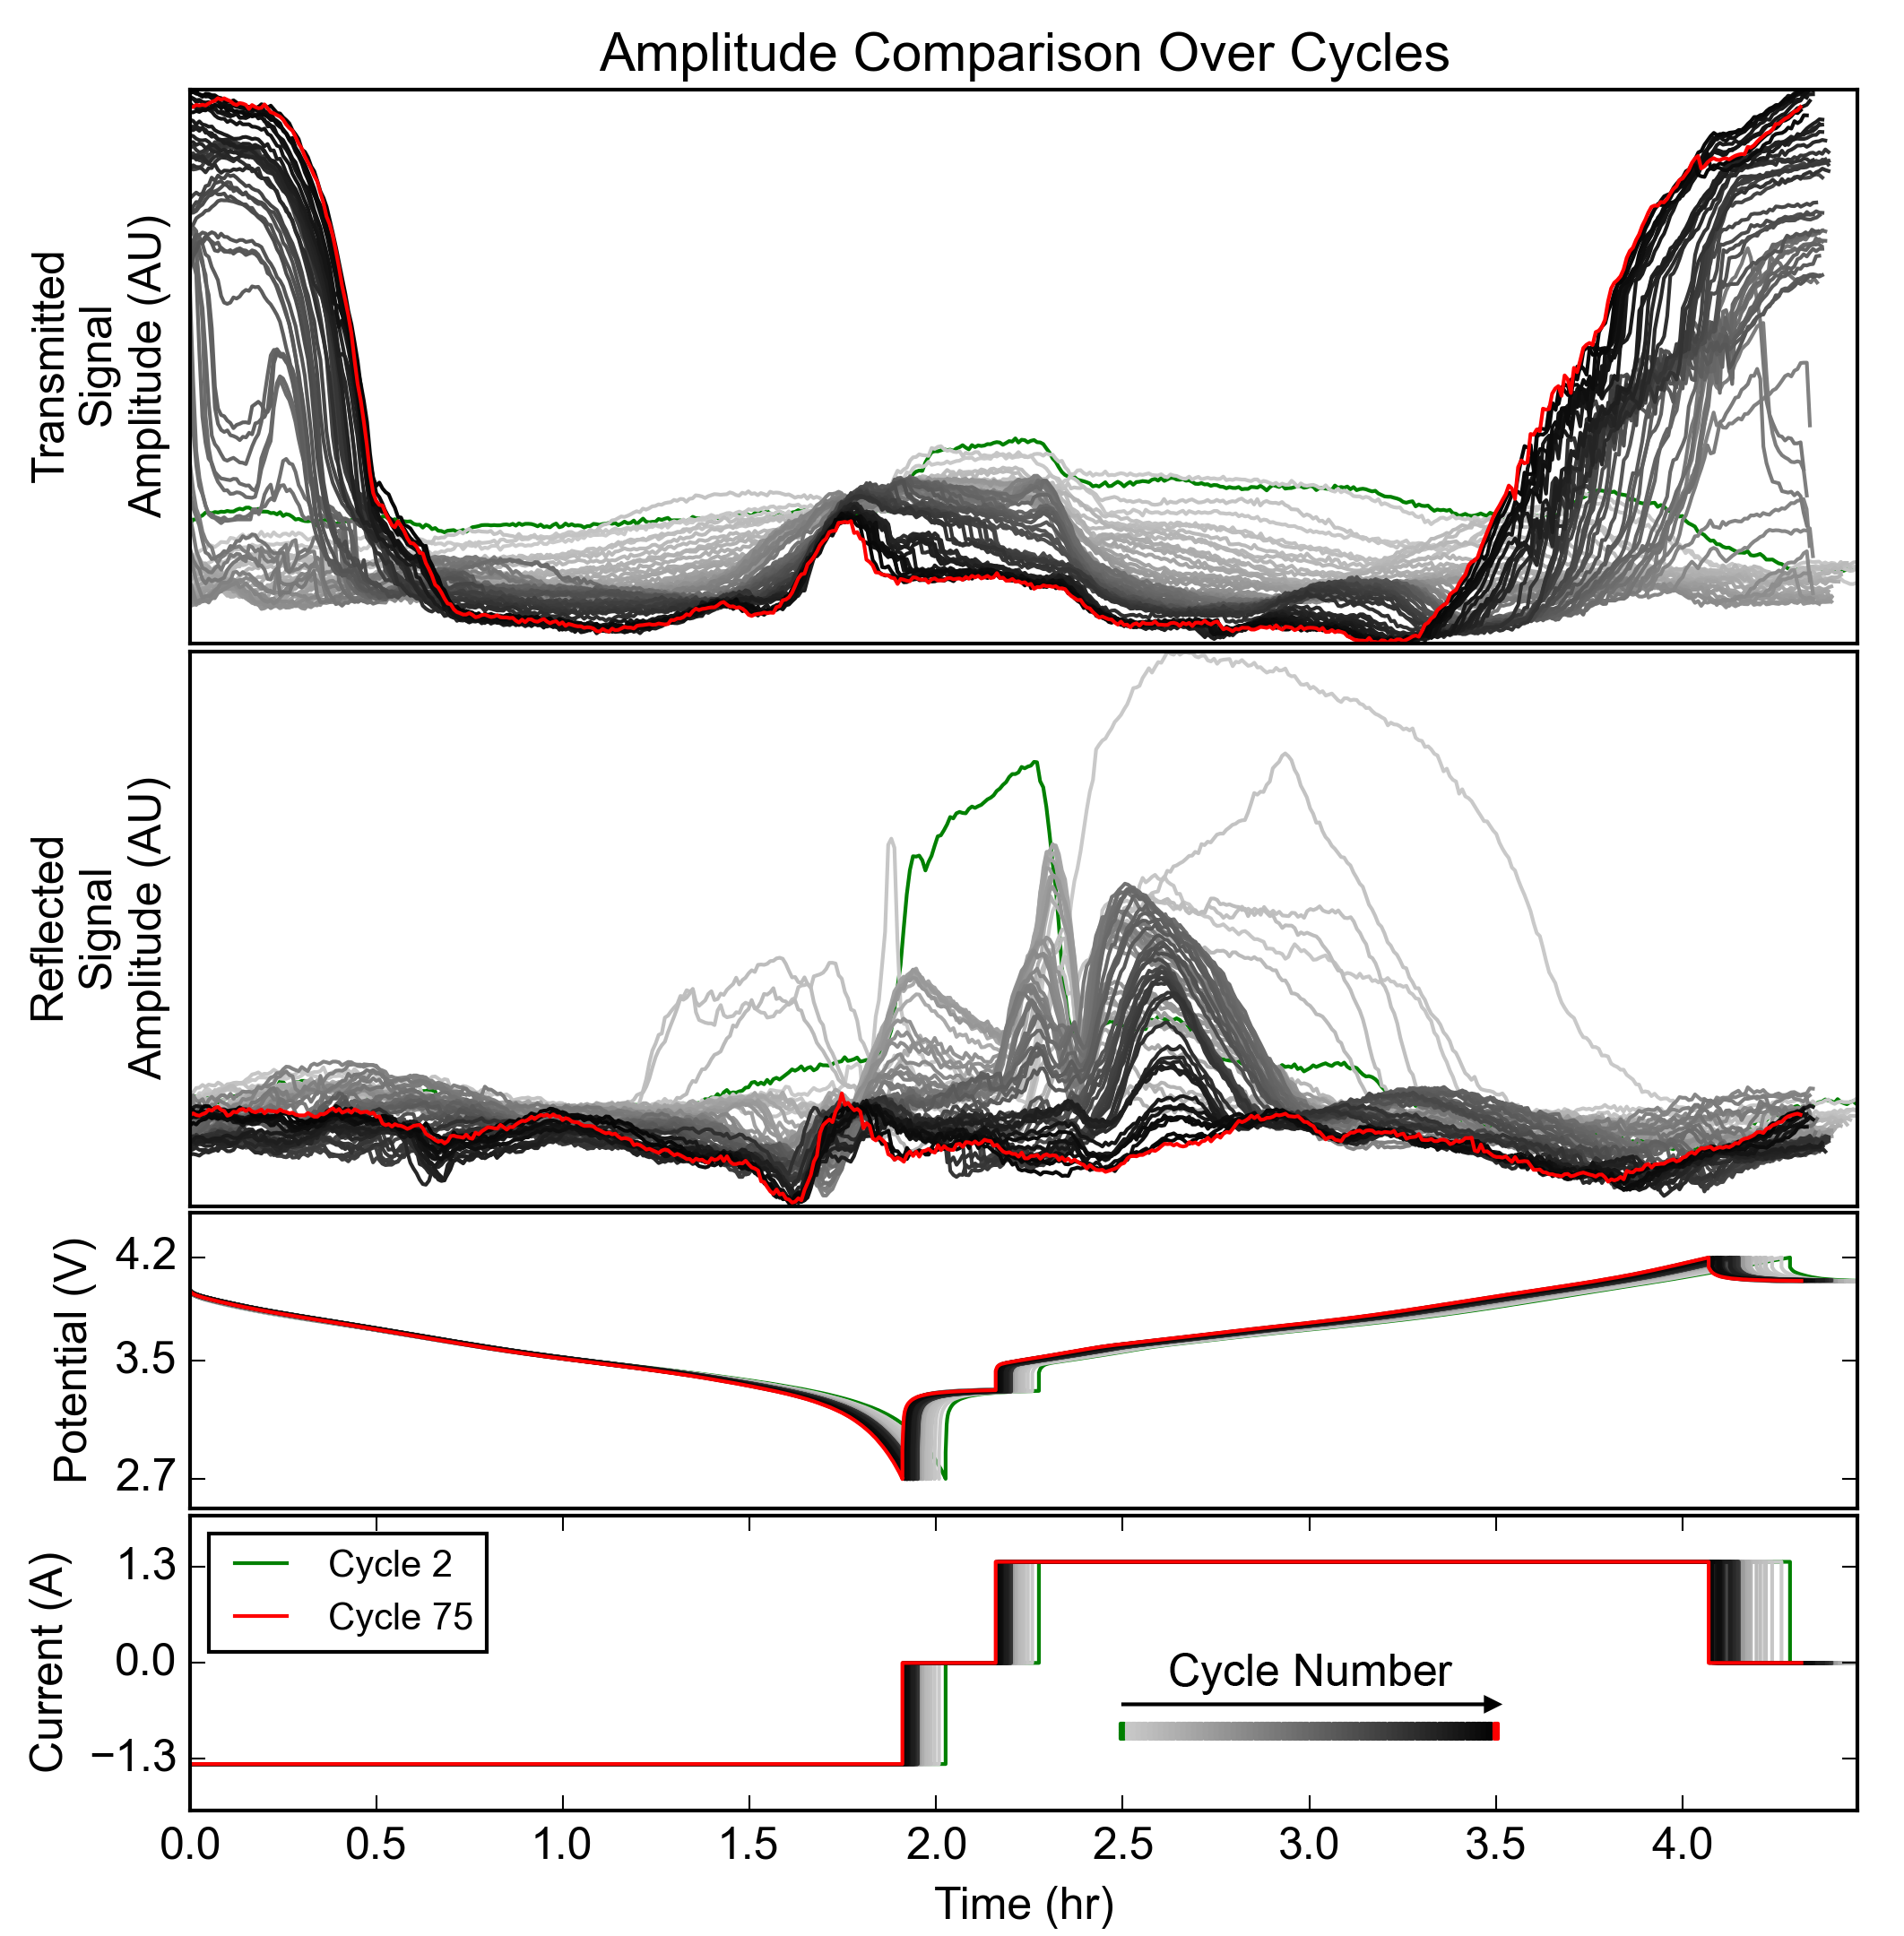
\includegraphics[width=\textwidth]{ch4-bw/images/ncacycle.png}
    \caption[Cycle-to-cycle analysis of the acoustic behavior of an NCA/graphite 18650 cell.]{Cycle-to-cycle analysis of the acoustic behavior of an NCA/graphite 18650 cell. Evolution of (from top) the transmitted and reflected signal amplitudes, cell potential, and applied current as a function of cycling time for cycles 2 through 75 from the acoustic/electrochemical data in Fig. 4. For each plot, the first cycle is indicated in green, with subsequent cycles shown as progressively darker shades of grey and the final cycle indicated in red.}
    \label{fig:ncacycle}
\end{figure}

\clearpage

While our computational model generally describes the experimentally observed acoustic phenomena in lithium-ion batteries, there are notable differences that demand further investigation. First, the 90\degree phase shift between reflected and transmitted waves in the model is not seen in either lithium-ion cell tested; we believe an additional layer may be present in the cells that may ``rephase" the signal, however a more detailed consideration of individual layer effects is required. Second, our model did not account for modulus changes within the electrodes during cycling (though they are likely present), which probably contributes to the more dramatic shifts in acoustic signal delay and attenuation. Third, our model only considered density changes due to lithium intercalation and de-intercalation; in reality, density and modulus changes due to phase transformation, staging effects, etc. also need to be considered. Fourth, due to the one-dimensional nature of our model, heterogeneities in current density throughout the electrodes during cycling were not accounted for. Furthermore, assumptions were made regarding electrode porosity and acoustic homogeneity. Nonetheless, the model presented herein does begin to describe the complex but repeatable acoustic response within the batteries. This is an important point that bears emphasizing: Though our model does not capture many of the detailed acoustic and electrochemical processes, it nevertheless captures much of the general behavior observed experimentally. This clearly shows the feasibility of the electrochemical-acoustic approach for SOC and SOC determination, and lays the groundwork for future studies.

\subsection{Preliminary ultrasonic ToF analysis of Zn/\ce{MnO2} alkaline AA cells}

\begin{figure}[htb]
  \centering
    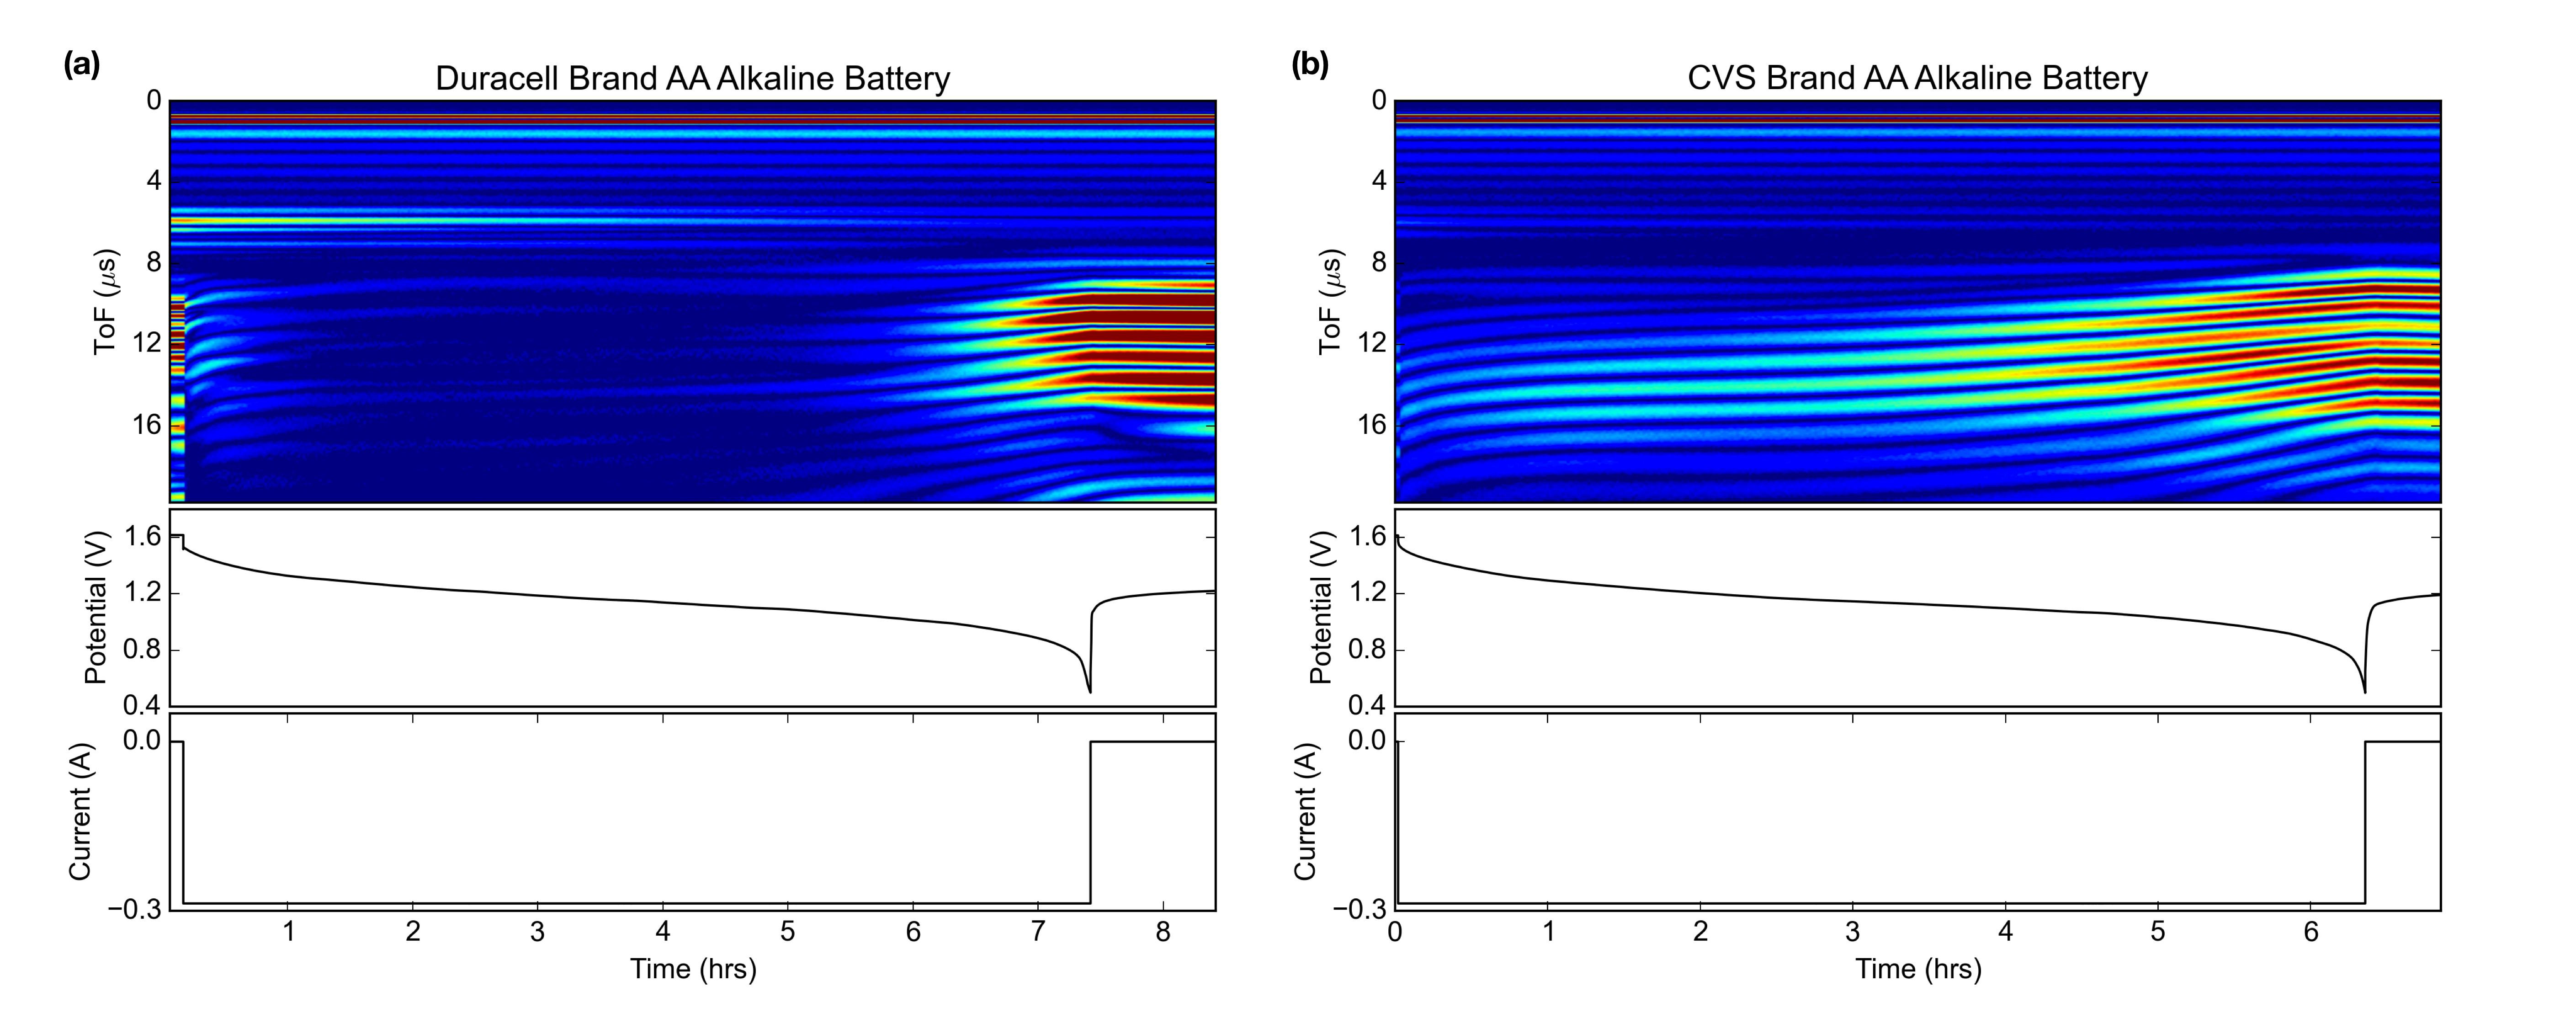
\includegraphics[width=\textwidth]{ch4-bw/images/aacomp.png}
    \caption[Acoustic behavior of two brands of alkaline AA cells.]{Acoustic behavior of two brands of alkaline AA cells. a) Transmission ToF map of an ultrasonic pulse in a Duracell alkaline AA, with the corresponding cell potential and current profiles. b) Transmission ToF map of an ultrasonic pulse in a CVS brand alkaline AA, with the corresponding cell potential and current profiles. Both cells were discharged at 280 mA, corresponding to a C/10 rate.}
    \label{fig:aacomp}
\end{figure}

Ultrasonic time of flight experiments were also performed on commercial Zn-\ce{MnO2} alkaline AA cells from two different manufacturers (Duracell and CVS) during galvanostatic discharge at 400 mA. The data and analysis presented here act as a foundation for the more in-depth analysis on ultrasonic interrogation of alkaline AA cells presented in Chapter~\ref{ch:alkbw}. As shown in Fig.~\ref{fig:aacomp}, the two alkaline cells exhibited similar overall acoustic responses, however there are notable differences between them: The transmitted signal of the Duracell was initially greater than that of the CVS cell. We attribute this to the Duracell battery design, specifically to the delamination of the Duralock\textsuperscript{TM} corrosion protection layer. This proprietary polymeric coating on the Zn anode particles increases mechanical contact between them and results in the larger initial transmission signal compared to the CVS cell. When the discharge current was applied, the acoustic signal attenuated in both the Duracell and CVS brand batteries; this effect was more pronounced in the Duracell, as demonstrated in Fig.~\ref{fig:bwbrandcomp}.

\begin{figure}[htb]
  \centering
    \includegraphics[width=\textwidth]{ch4-bw/images/brandcomp.png}
    \caption[Acoustic comparison of Duracell and CVS pharmacy brand AA alkaline AA batteries.]{Acoustic comparison of Duracell and CVS pharmacy brand AA alkaline AA batteries discharged at 400 mA. \textbf{Left:} Duracell ToF map. \textbf{Right:} CVS ToF map.}
    \label{fig:bwbrandcomp}
\end{figure}

In both cells we believe this initial attenuation is due in part to the nature of the discharge reaction: in an alkaline (e.g. KOH) electrolyte, solid Zn is stripped from the surface of individual particles and aqueous zincate \ce{(Zn(OH)4^{2-})} ions form. This causes the Zn particle network to become less packed, which in turn attenuates the acoustic signal. In the Duracell, though, we also attribute some of the acoustic attenuation to the disintegration of the Duralock\textsuperscript{TM} coating. This is corroborated by EIS, shown in Fig.~\ref{fig:bweis}, in the form of a 2 order-of-magnitude drop in total cell impedance after the onset of discharge. Subsequent EIS scans do not show appreciable changes based on state of charge.

\begin{figure}[htb]
  \centering
    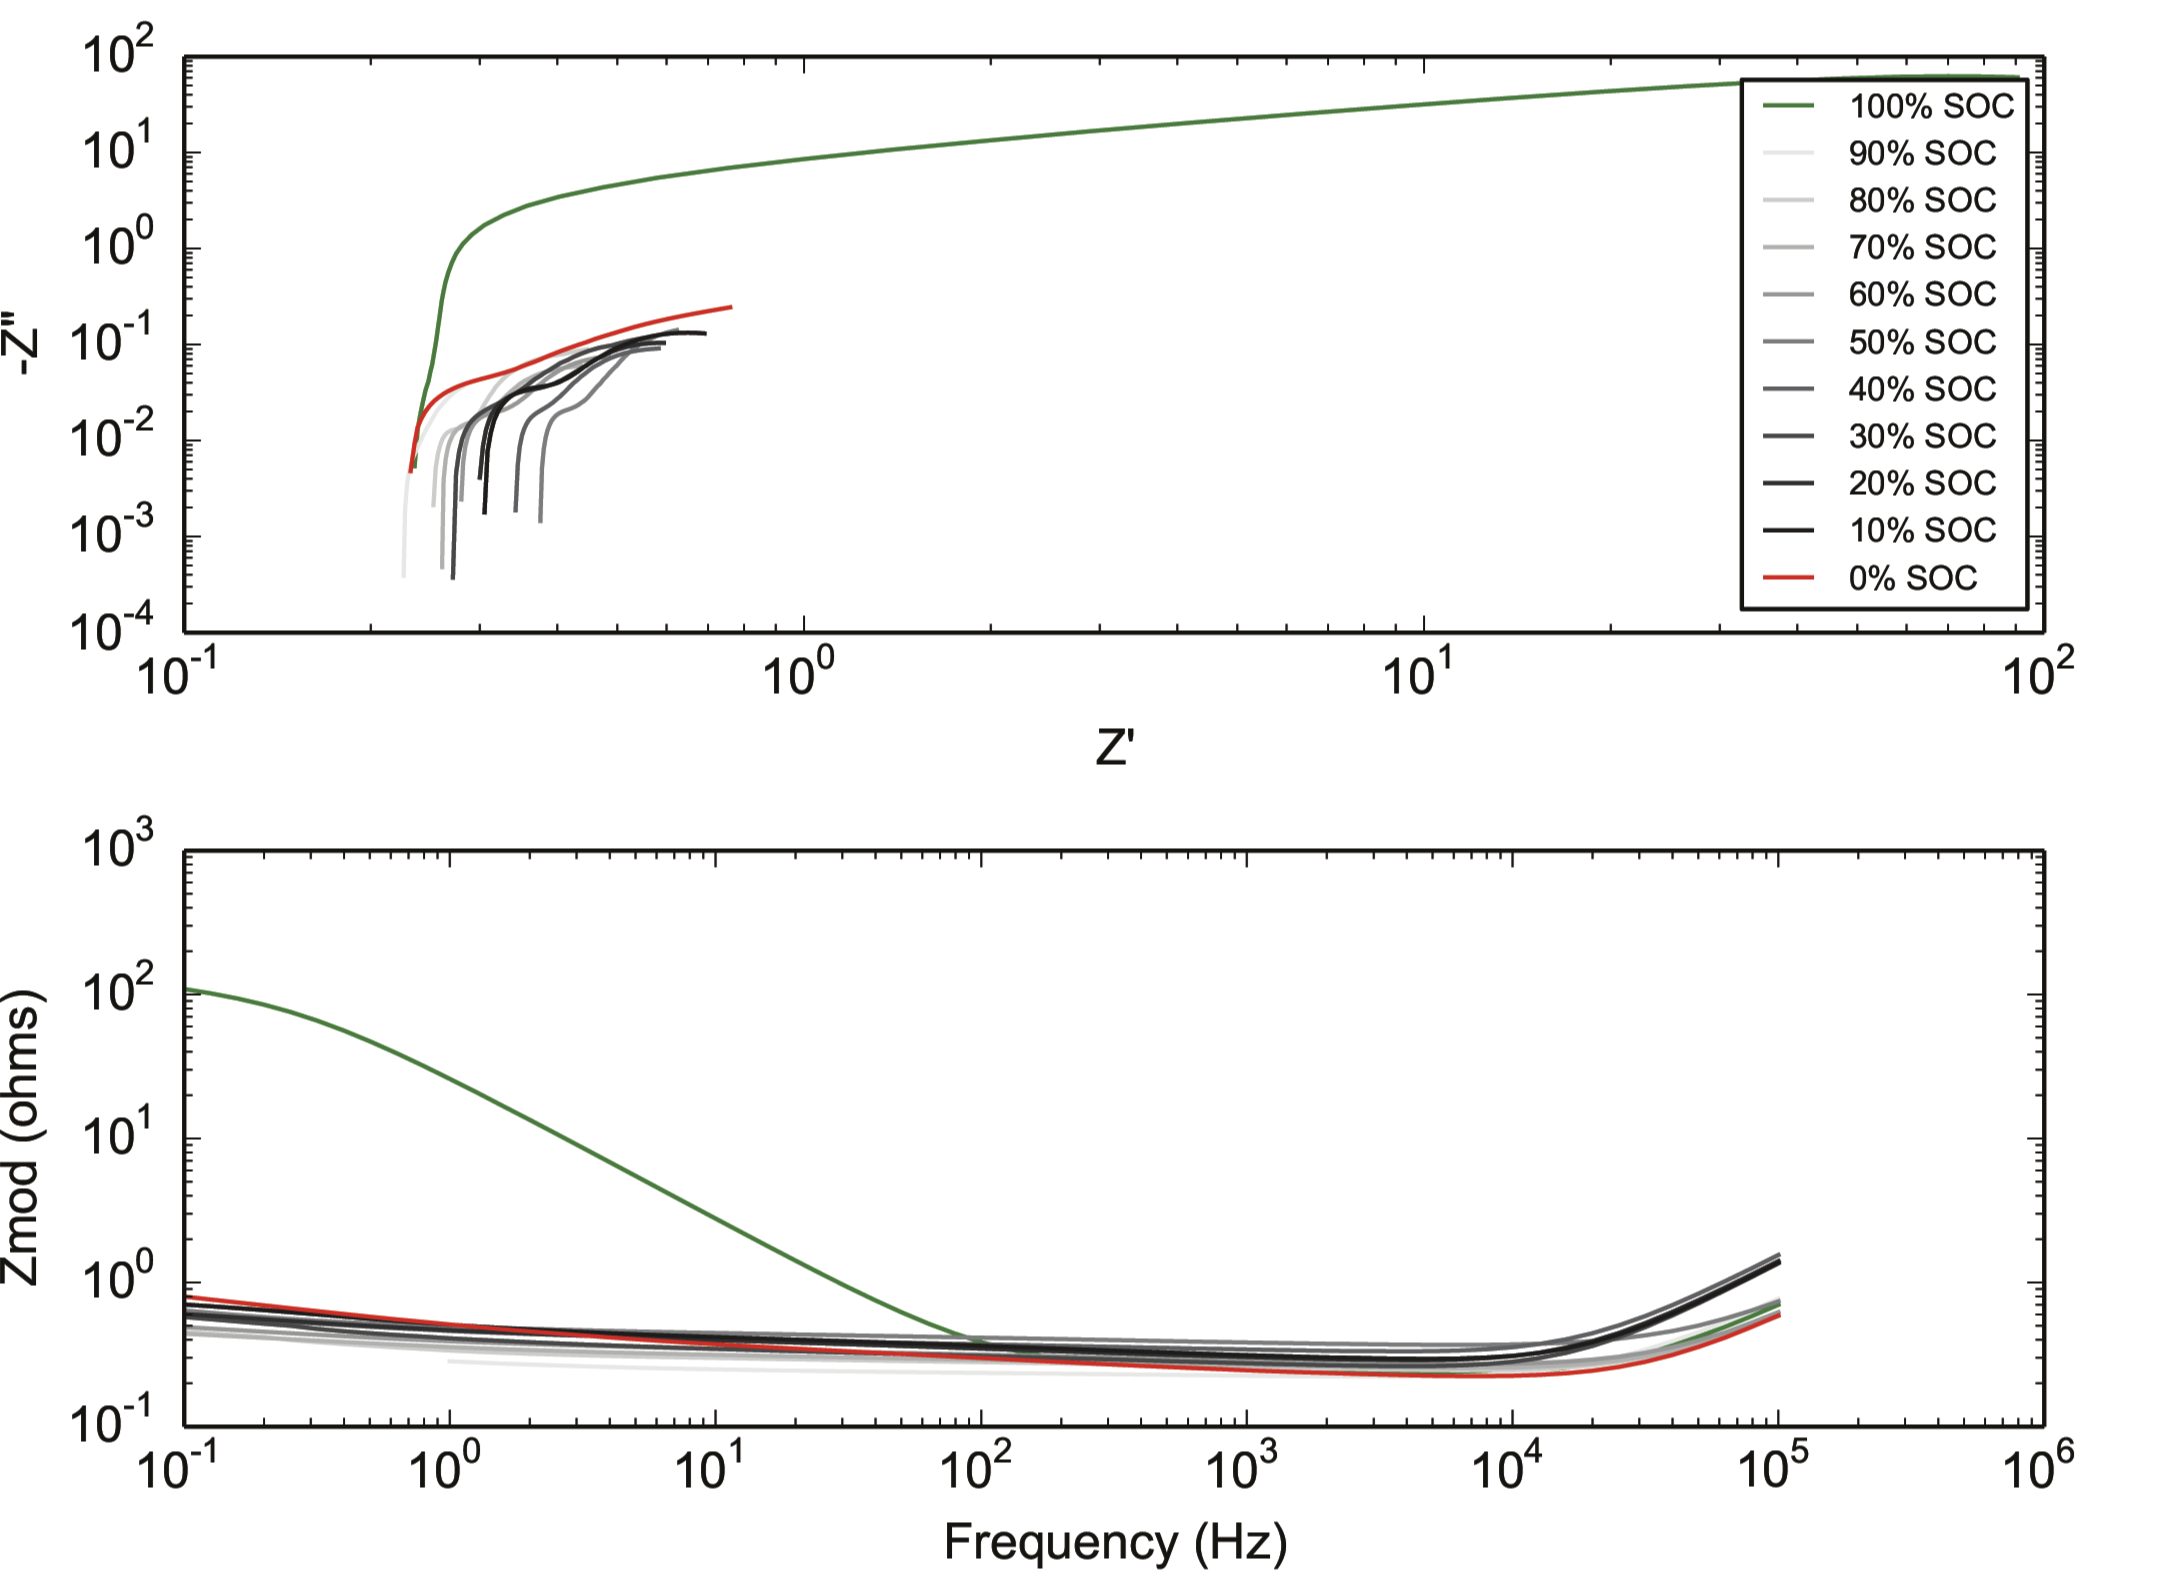
\includegraphics[width=\textwidth]{ch4-bw/images/eis.png}
    \caption[Electrochemical impedance spectra for a Duracell AA alkaline battery.]{Electrochemical impedance spectra for a Duracell AA alkaline battery as a function of state of charge. \textbf{Top:} Nyquist plot. \textbf{Bottom:} Bode plot.}
    \label{fig:bweis}
\end{figure}

As discharge continues in both cells, the transmission peak traces between 8 and 20 µs undergo shifts in ToF that follow Nernstian-like patterns, similar to the changes in cell potentials, and the acoustic signal intensities are greatly enhanced by the end of discharge. This is likely due to the formation of solid ZnO as the the saturation limit of \ce{Zn(OH)4^{2-}} is reached.~\cite{Dirkse1954-di,Szpak1979-qy} Eventually, near the end of discharge, the ZnO creates a percolated network of ZnO within the anode, causing the transmitted signal to increase dramatically.~\cite{Bhadra2015-aq} In the Duracell, however, we note that after the current is applied the signal intensity decreases until about halfway through the discharge step before it begins to increase. This is distinct from the CVS cell, in which (after the initial attenuation) the transmitted signal increases monotonically throughout discharge. We believe this difference is a result of the Duralock\textsuperscript{TM} corrosion protection layer as well as proprietary electrolyte additives used by Duracell to prevent corrosion and increase ZnO solubility. Indeed, upon dissection of fresh batteries, we found Zn from the Duracell to be more lustrous than that from the CVS cell, indicating less ZnO in the Duracell initially. 

There is also a set of ToF peaks between 4 and 8 µs that is more pronounced in the Duracell battery than in the CVS battery. We attribute this observation to differences in the cathode materials; the Duracell cathode appears to have smaller, more densely packed particles than the CVS cathode, as shown in confocal microscope images in Fig.~\ref{fig:bwcathode}, which would result in a more mechanically-connected network. In both cells, these peaks gradually fade in intensity (but do not shift in ToF) during discharge. This is possibly due to the expulsion of aqueous electrolyte from the anode to the cathode during discharge, which has been observed via in-situ neutron tomography by Riley et. al.~\cite{Riley2010-ur} The increase in cathode water content would cause the relevant transmission peaks to attenuate relative to a drier cathode. After discharge, the relaxation behavior appears to be similar for both cells. These results are particularly noteworthy because they show that acoustic time of flight measurements can be sensitive enough to detect differences in manufacturing processes between multiple brands of the same battery chemistry. This detection ability is further investigated in Chapter~\ref{ch:alkbw}.

\begin{figure}[htb]
  \centering
    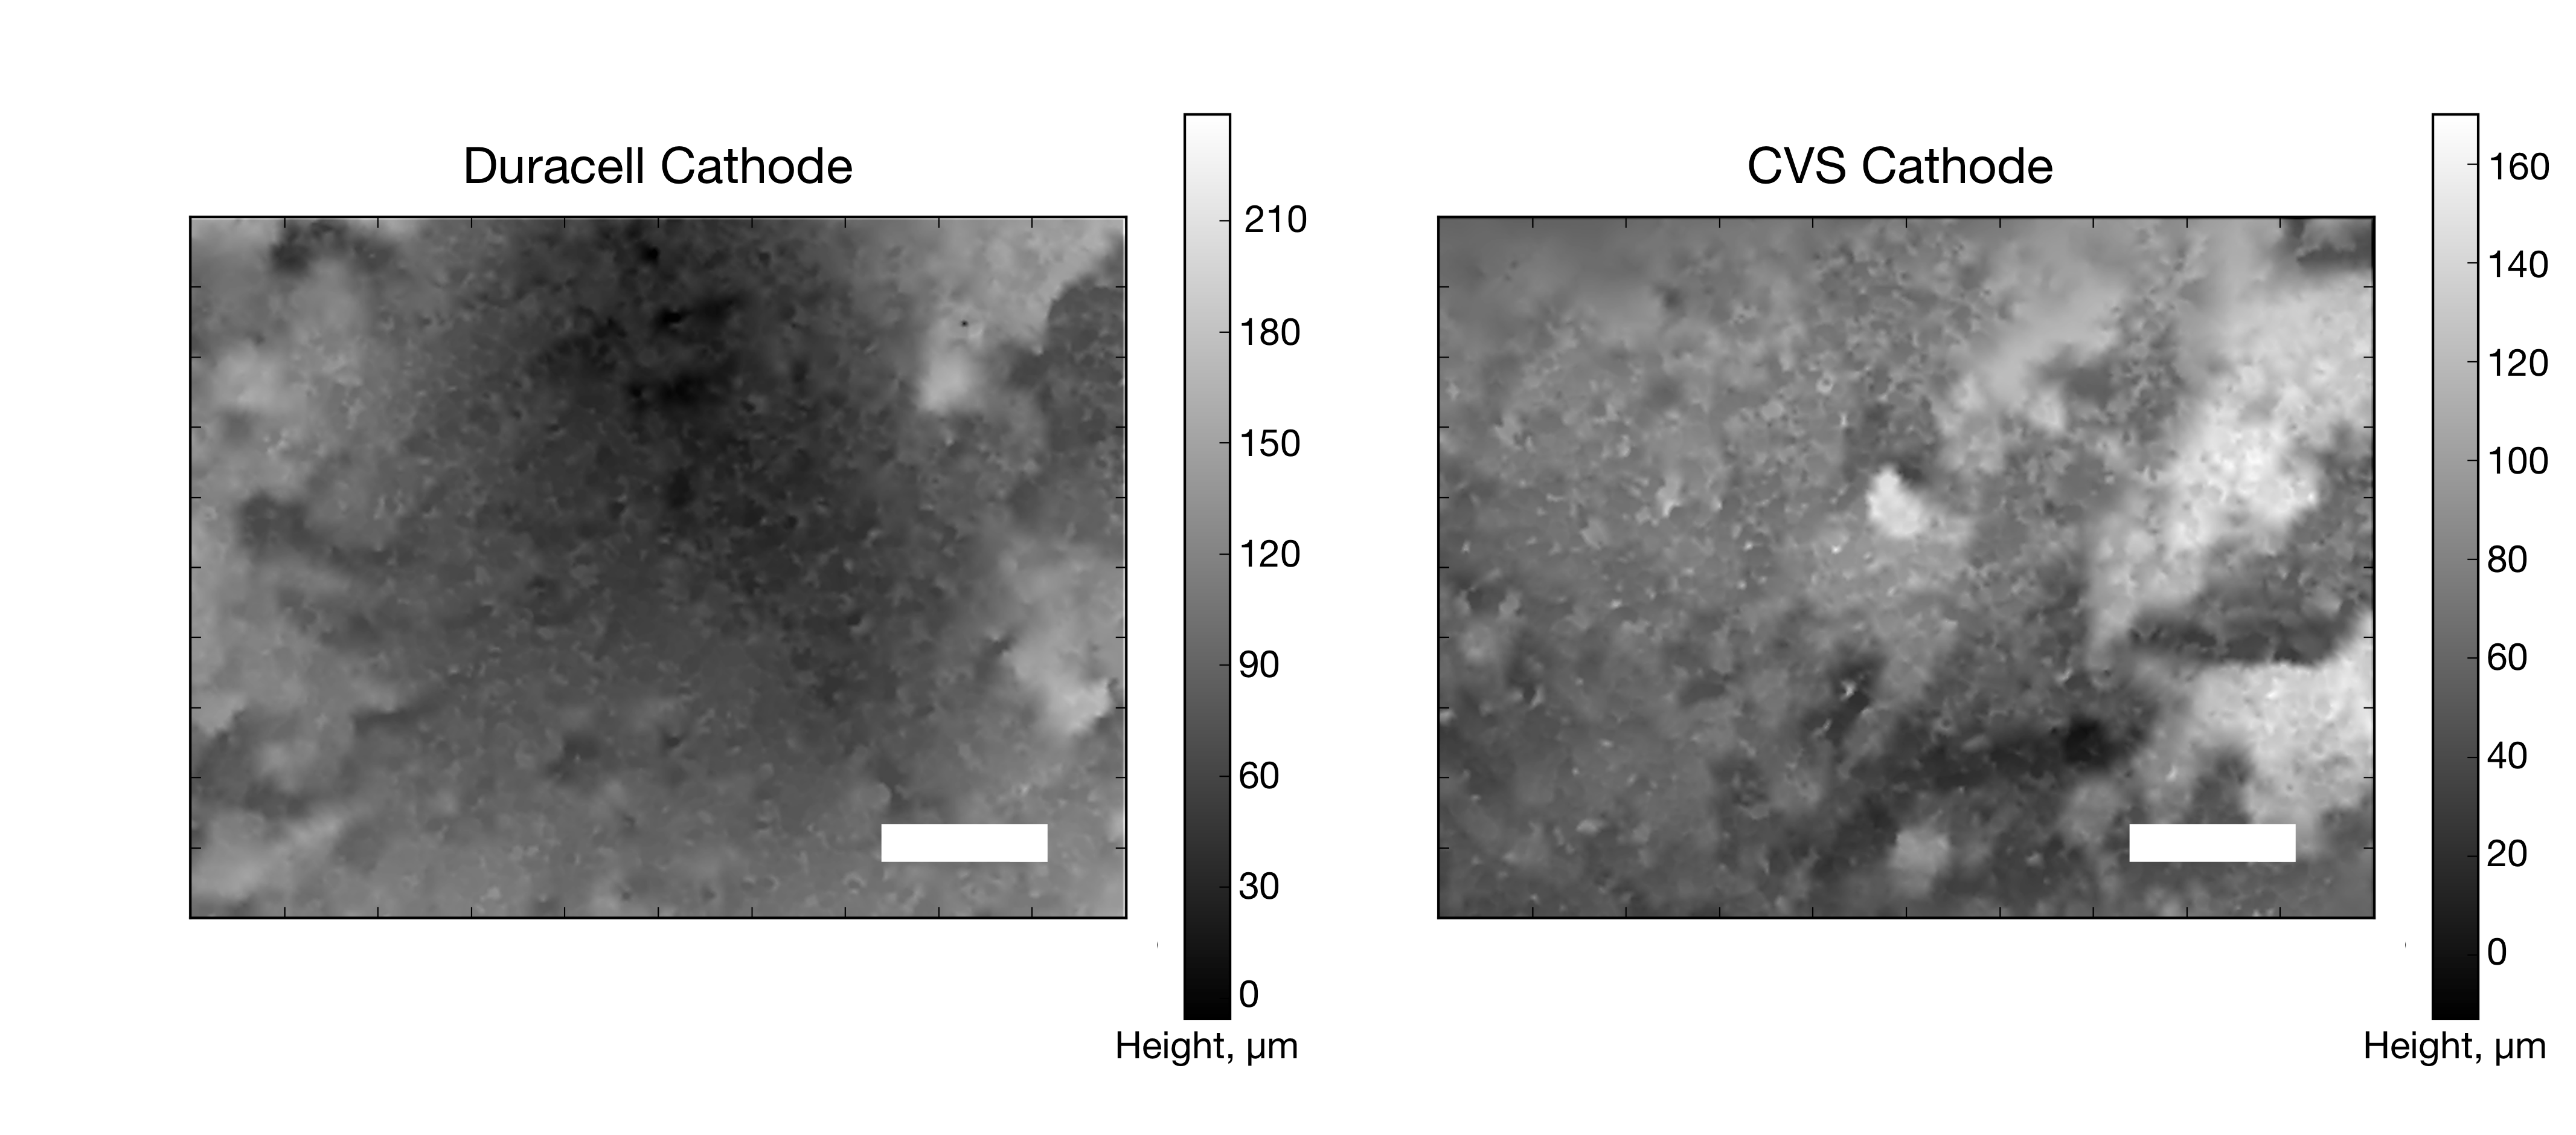
\includegraphics[width=\textwidth]{ch4-bw/images/cathode.png}
    \caption[Confocal microscope images of Duracell and CVS brand Alkaline AA cathodes.]{Confocal microscope images of Duracell and CVS brand Alkaline AA cathodes. \textbf{Left:} Duracell brand cathode. \textbf{Right:} CVS brand cathode. Scale bars are 250 μm for both.}
    \label{fig:bwcathode}
\end{figure}

To demonstrate the effect of discharge current on the acoustic behavior of alkaline batteries, Duracells were discharged at different rates (C/20, C/10, C/3). As shown in Fig.~\ref{fig:bwratecomp}, the cells show a marked difference in their acoustic transmission profiles as a function of discharge rate. The morphology and spatial distribution of ZnO in alkaline batteries is known to depend on discharge rate, as shown by Horn et al.,~\cite{horn} so the different ToF profiles are probably due to the influence of discharge rate on formation of ZnO and thus mechanical properties of the full cell. Higher discharge rates result in ZnO forming predominantly in the regions closest to the anode/separator interface, while lower discharge rates result in a more uniform distribution of ZnO formation throughout the anode. Thus, cells that are discharged more slowly develop a ZnO network that is more percolated (and thus transmits sound more readily) than cells that are discharged more quickly.~\cite{Bhadra2015-aq} A detailed understanding of the structural and mechanical changes that are responsible for the ToF behavior in alkaline cells will be addressed further in Chapter~\ref{ch:alkbw}.

\begin{figure}[htb]
  \centering
    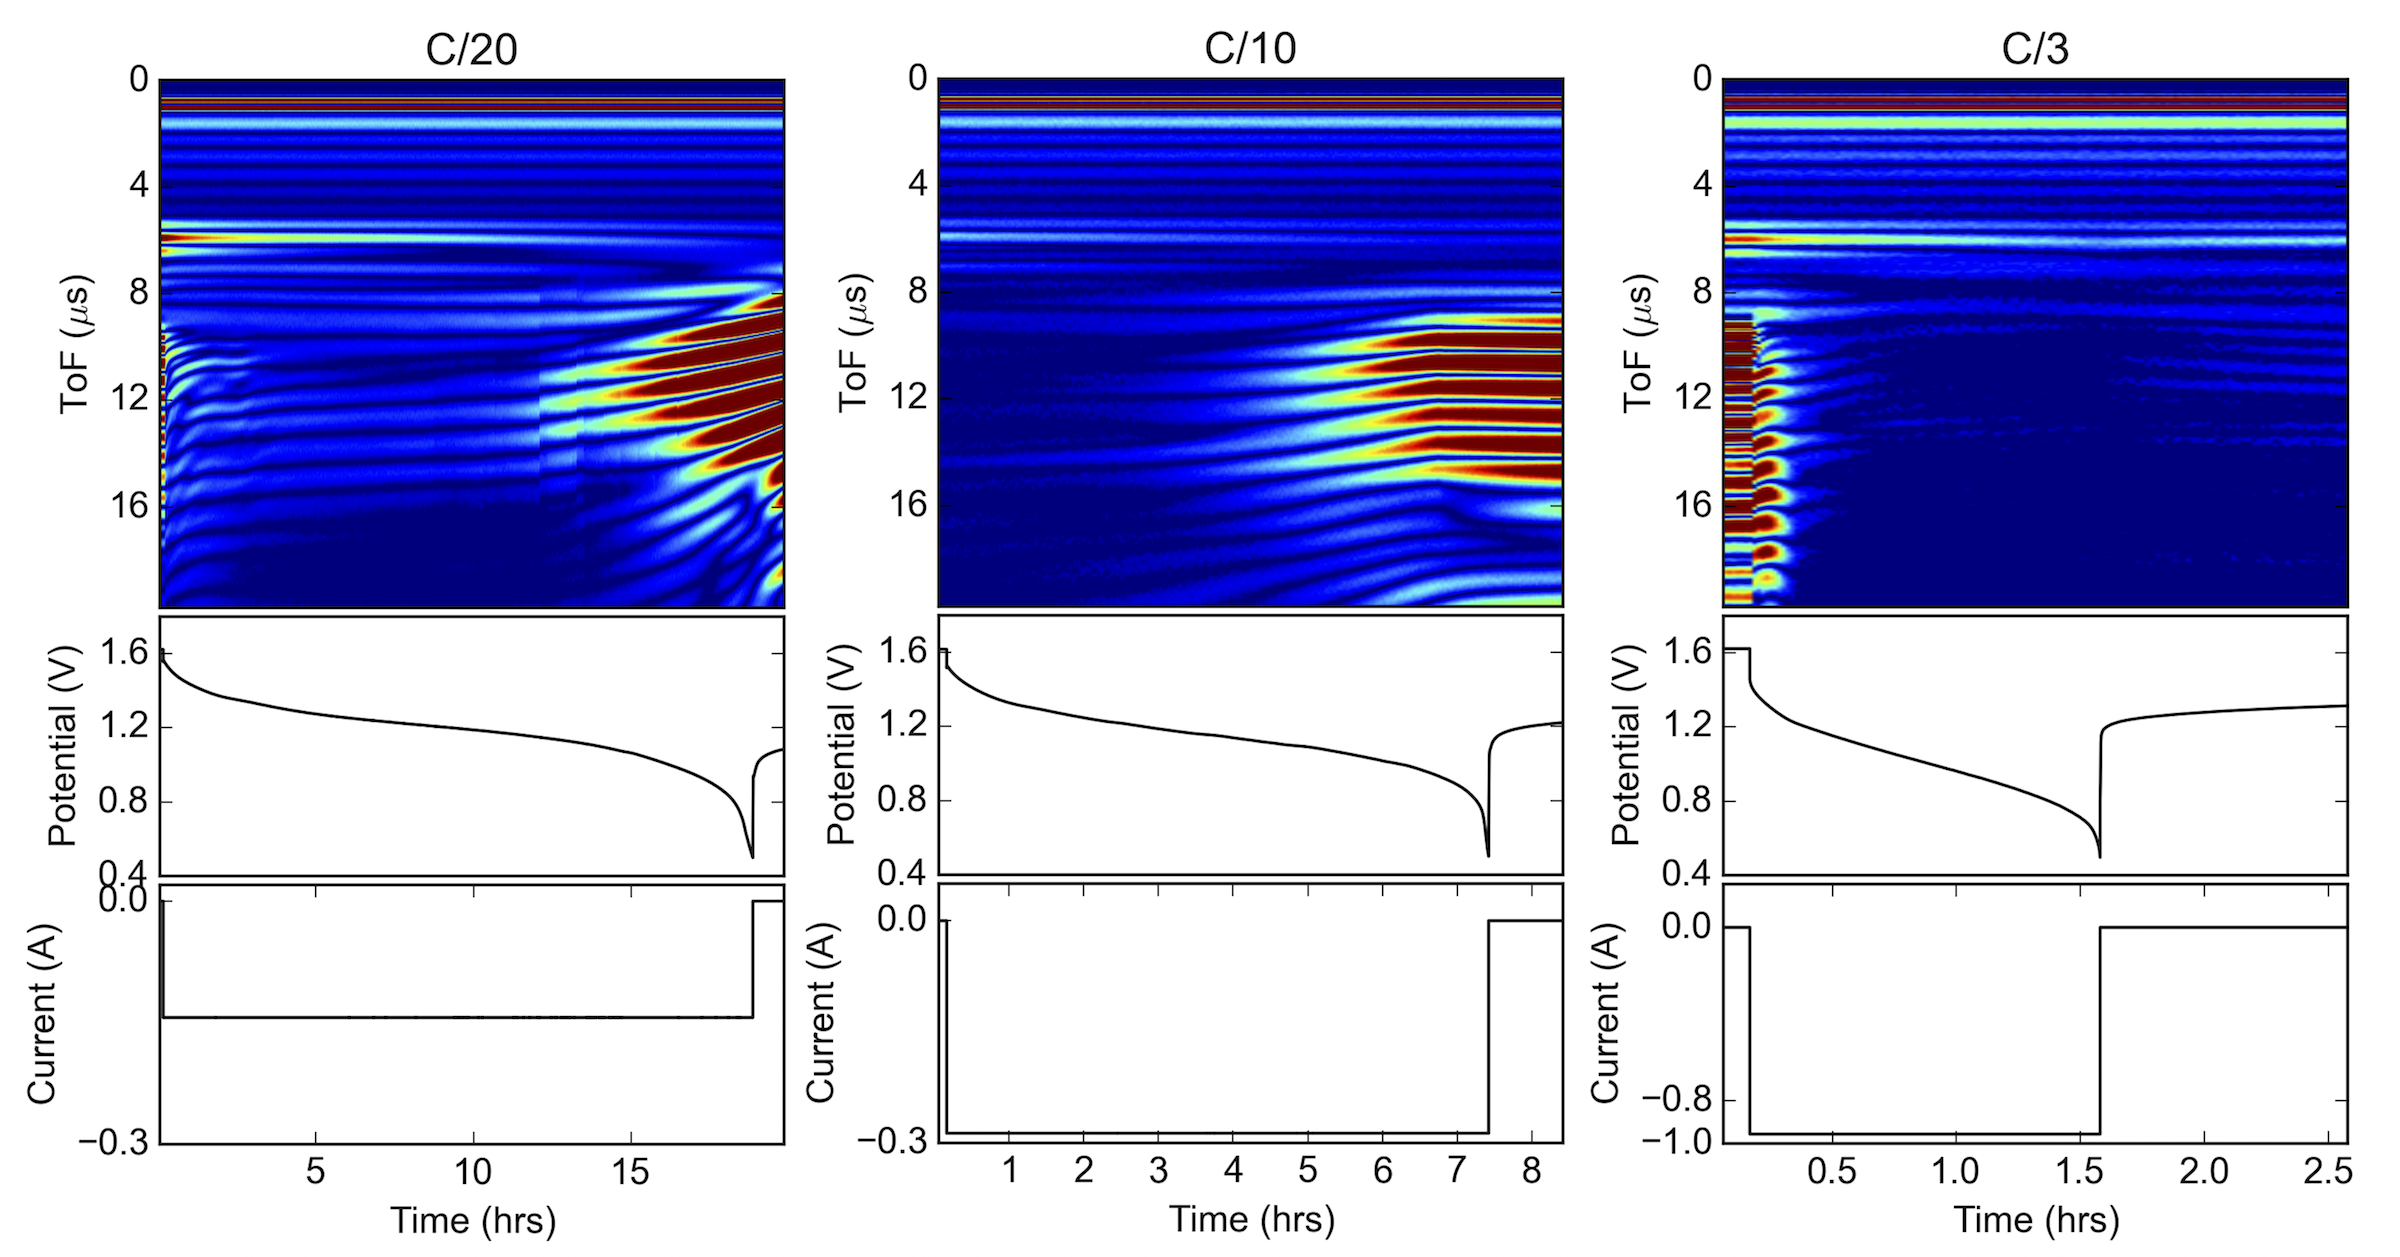
\includegraphics[width=\textwidth]{ch4-bw/images/ratecomp.png}
    \caption[Acoustic evolution of a Duracell AA alkaline battery at multiple discharge rates.]{Acoustic evolution of a Duracell AA alkaline battery at multiple discharge rates. \textbf{From left to right:}  C /20, C/10, C/3.}
    \label{fig:bwratecomp}
\end{figure}




